%%%%%%%%%%%%%%%%%%%%%%%%%%%%%%%%%%%%%%%%%%%%%%%%%%%%%%%%%%%%%%%%%%%%%%%%%%
% File: week7_stencil.tex
% Authors: Nicholas Chaimov
% Date: March 3, 2014
% Description: 
%%%%%%%%%%%%%%%%%%%%%%%%%%%%%%%%%%%%%%%%%%%%%%%%%%%%%%%%%%%%%%%%%%%%%%%%%%

%<<<<<<<<<<<<<<<<<<<<<<<<<<<<<<<<<<<<<<<<<<<<<<<<<<<<<<<<<<<<<<<<<<<<<<<<<<<<<%
% Document package information
%>>>>>>>>>>>>>>>>>>>>>>>>>>>>>>>>>>>>>>>>>>>>>>>>>>>>>>>>>>>>>>>>>>>>>>>>>>>>>%
\documentclass[xcolor=dvipsnames]{beamer} 
%%%%%%%%%%%%%%%%%%%%%%%%%%%%%%%%%%%%%%%%%%%%%%%%%%%%%%%%%%%%%%%%%%%%%%%%%%
% File: _TeXdefs.tex
% Author: James Kress
% Date: January 25, 2014
% Description: A tex file containing the \usepackage declarations, and
%			   other document critial style settings.
%%%%%%%%%%%%%%%%%%%%%%%%%%%%%%%%%%%%%%%%%%%%%%%%%%%%%%%%%%%%%%%%%%%%%%%%%%

%-----------Package imports
\usepackage{graphicx}
\usepackage{pgfpages}
\usepackage{tikz}
\usepackage{latexsym}
\usepackage{verbatim}
%//////////END package imports


%----------Style elements
\useoutertheme{infolines} 
\usetheme{Frankfurt} 
\usepackage{../theme/beamercolorthemeoregon}
\setbeamertemplate{sections/subsections in toc}[default]
\setbeamertemplate{footline}
{
\leavevmode%
  \hbox{%
  \begin{beamercolorbox}[wd=.3\paperwidth,ht=2.25ex,dp=.75ex,center]{institute in head/foot}%
    \usebeamerfont{institute in head/foot}\insertshortinstitute
  \end{beamercolorbox}%
    \begin{beamercolorbox}[wd=.4\paperwidth,ht=2.25ex,dp=.75ex,center]{title in head/foot}%
      \usebeamerfont{title in head/foot}\insertshorttitle
    \end{beamercolorbox}%
  \begin{beamercolorbox}[wd=.3\paperwidth,ht=2.25ex,dp=.75ex,center]{date in head/foot}%
    \usebeamerfont{date in head/foot}\insertshortdate\hspace*{3em}
    \insertframenumber{} / \inserttotalframenumber\hspace*{1ex}
  \end{beamercolorbox}}%
  \vskip0pt%
}
%/////////END style elements


%---------Command Declarations
\DeclareGraphicsExtensions{.pdf, .jpeg, .png, .jpg}
\graphicspath{ {../images/} }
\newcommand{\className}{\text{CIS 410/510} \\ \text{Parallel Computing}}
\newcommand{\departmentName}{\textit{Department of Computer and 
									Information Science \\ University of Oregon}}
%/////////END command declarations


%---------Setup pdf properties
\hypersetup{
	pdfusetitle=true,
    bookmarks=true,         	% show bookmarks bar?
    unicode=false,          	% non-Latin characters in Acrobat’s bookmarks
    pdftoolbar=true,        	% show Acrobat’s toolbar?
    pdfmenubar=true,        	% show Acrobat’s menu?
    pdffitwindow=false,     	% window fit to page when opened
    pdfstartview={Fit},   		% fits the width of the page to the window    
    pdfauthor={},     % author
    pdfsubject={Parallel Programming},   	% subject of the document
    pdfcreator={},   			% creator of the document
    pdfproducer={}, 			% producer of the document
    pdfkeywords={University of Oregon, parallel programming}, 
    pdfnewwindow=true,      	% links in new window
    colorlinks=true,       		% false: boxed links; true: colored links
    linkcolor=white,          	% color of internal links
    hidelinks,
    citecolor=green,        	% color of links to bibliography
    filecolor=magenta,      	% color of file links
    urlcolor=cyan,           	% color of external links
    linktoc=page,
    pageanchor = true
}
%//////////END setup pdf properties


%END ALL


%<<<<<<<<<<<<<<<<<<<<<<<<<<<<<<<<<<<<<<<<<<<<<<<<<<<<<<<<<<<<<<<<<<<<<<<<<<<<<%
% END Document package information
%>>>>>>>>>>>>>>>>>>>>>>>>>>>>>>>>>>>>>>>>>>>>>>>>>>>>>>>>>>>>>>>>>>>>>>>>>>>>>%

%=============================================================================%
% Begining: Title Page Material
%=============================================================================%
\begin{document}
	\title[Stencil Pattern]{Stencil Pattern}
	\author[]{\className}
	\institute[\className]{\departmentName}
	\date{} 

	\titlegraphic{\centering 
		$\vcenter{\hbox{
\includegraphics[height=.31in,width=2.0in]{oregonLogo}}}$
	}

	\begin{frame}
		\maketitle
	\end{frame}
	
	\begin{frame}{Developer Training}
		\begin{center}
			
\includegraphics[width=0.4\textwidth]{images/OSNAP_logo} 
			
			Stencil Pattern
			
			Automated UFO Detection
		\end{center}
	\end{frame}
	
	\begin{frame}{Automated UFO Detection}
		\begin{columns}
			\begin{column}{0.5\textwidth}
          Our current procedure for identifying spacecraft in space surveillance photos is to display a photo to an intern, who presses a button if a spacecraft is present. However, we are having severe problems with interns falling asleep or otherwise not paying attention.
          \\~\\
          We would like to automate the process of identifying spacecraft, in order to improve reliability and so that interns can be reassigned to coffee-making duties.
			\end{column}
			\begin{column}{0.5\textwidth}
				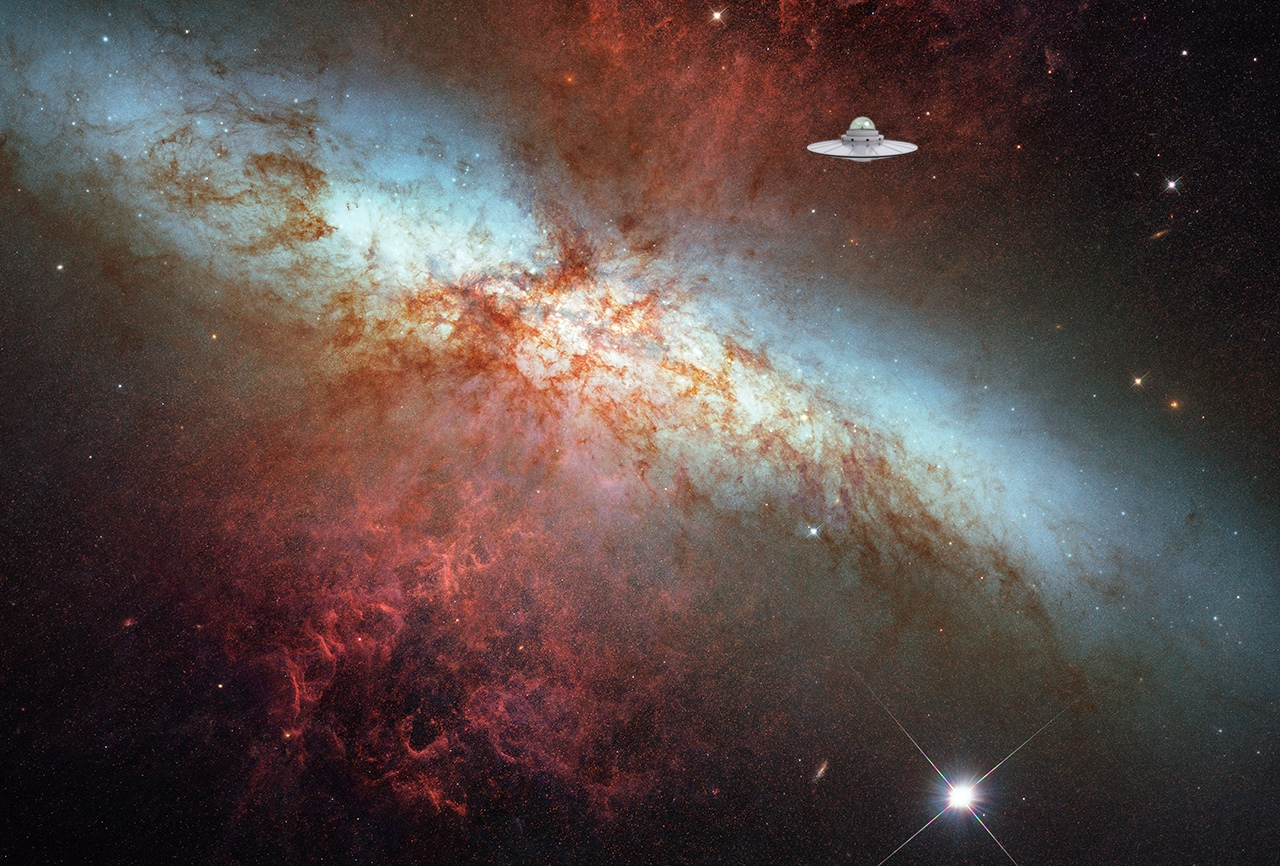
\includegraphics[width=\textwidth]{images/original}
			\end{column}
		\end{columns}
	\end{frame}
	
	\begin{frame}[t]{Edge Detection}
		\begin{center}
			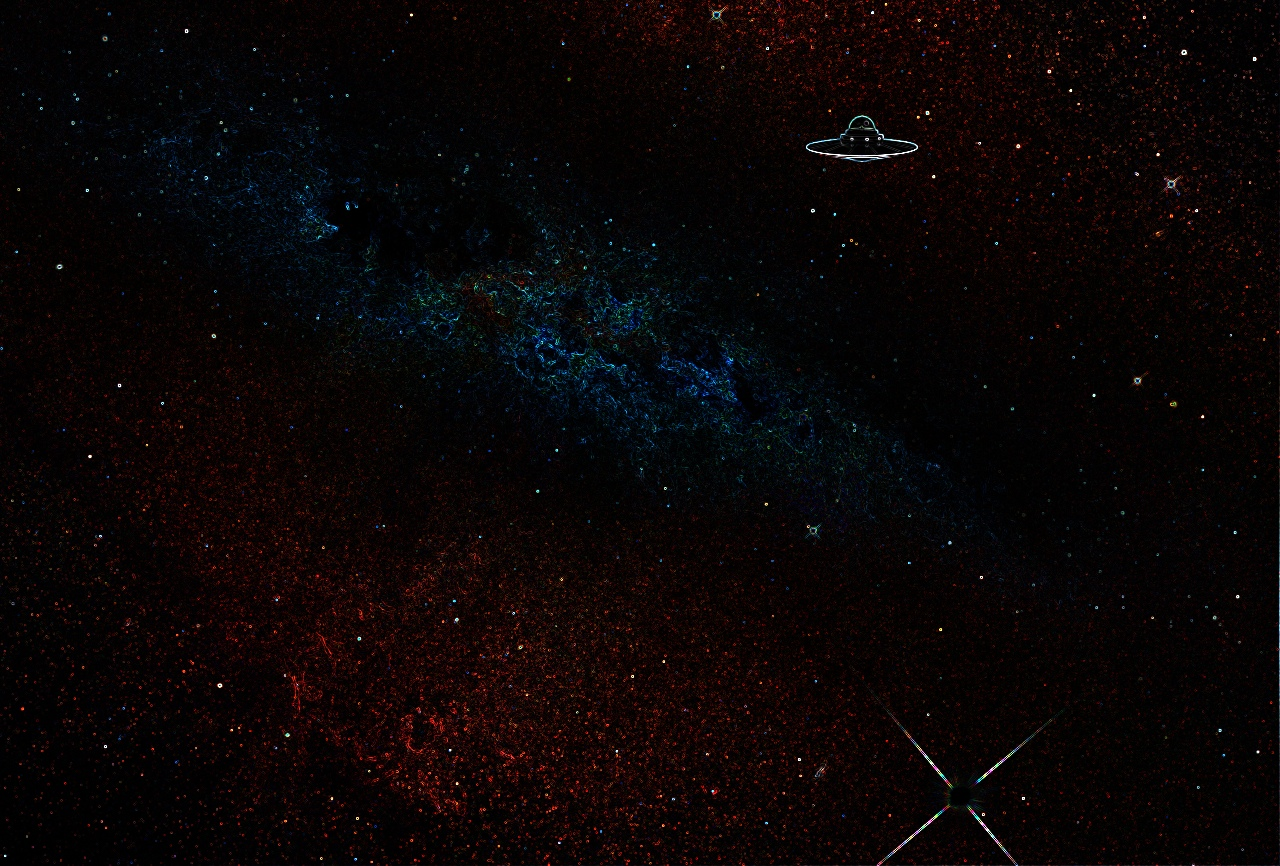
\includegraphics[width=0.65\textwidth]{images/edges}
			\\
			Our initial efforts at using edge detection successfully detects the spacecraft, but also produces a large amount of other edges resulting from stars, galaxies, pulsars, and other non-spacecraft objects.
		\end{center}
	\end{frame}

	\begin{frame}[t]{Gaussian Blur}
		\begin{columns}
			\begin{column}{0.5\textwidth}
				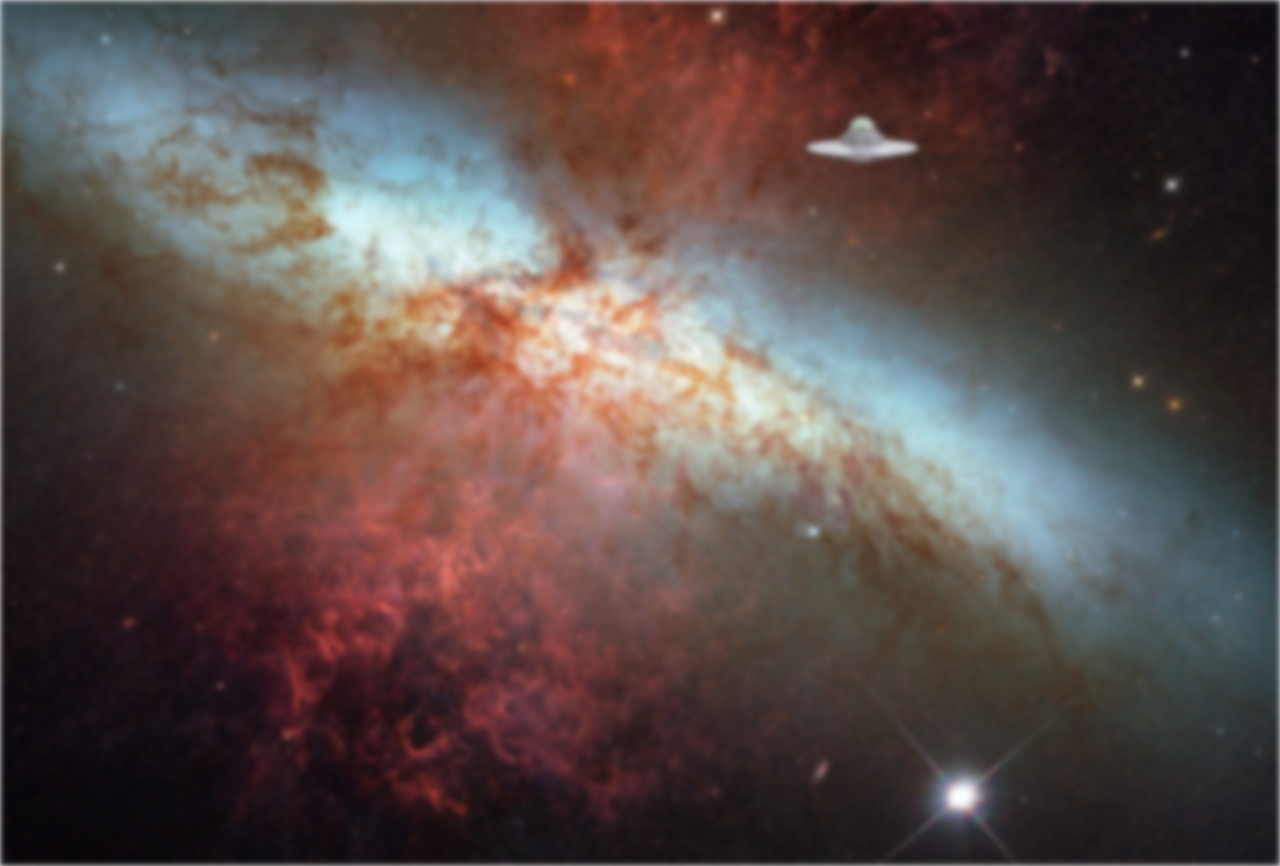
\includegraphics[width=\textwidth]{images/gaussian}
		\end{column}
		\begin{column}{0.5\textwidth}
				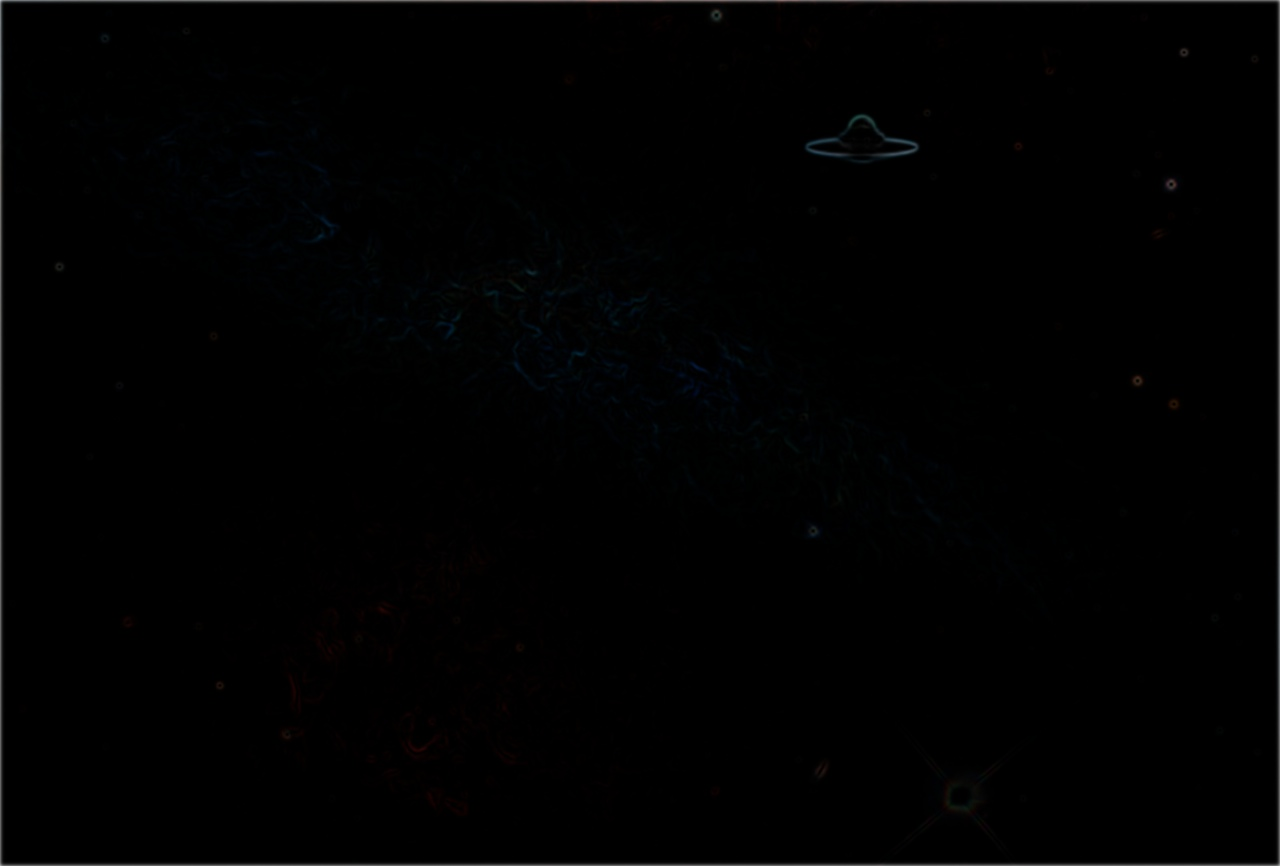
\includegraphics[width=\textwidth]{images/gaussian_edges}
		\end{column}
		\end{columns}
		~\\~\\
		Our current project is to apply a Gaussian blur filter to incoming images, softening the edges in order to isolate objects with sharper edges, such as UFOs.
	\end{frame}
	
	\begin{frame}[t]{Gaussian Blur Definition}
		A Gaussian blur is generated by, for each pixel, producing a weighted average of itself and adjacent pixels, where the weights are determined by a Gaussian function.\\
		\begin{equation*}
			G(x,y) = \frac{1}{2\pi \sigma^2} e^{-\frac{x^2 + y^2}{2 \sigma^2}}
		\end{equation*}
		~\\
		where $\sigma$ is the desired standard deviation for the Gaussian curve and $x$ and $y$ are distance from the center pixel. We generally consider only a limited neighborhood around each pixel, such as a $3 \times 3$ radius. These values can be pre-computed and then normalized so that they sum to one.
		\\~\\
		This is a \textbf{stencil} operation: each output depends on a ``neighborhood'' of inputs specified using a set of fixed offsets relative to the output position.
	\end{frame}
	%--- Next Frame ---%
%--- Next Frame ---%	
\end{document}
%END ALL

